Aplikacja została oparta o pusty projekt utworzony w frameworku Ionic. Ze względu na to, że Ionic opiera się AngularJS, zrezygnowano z jQuery na rzecz Angulara. Do obsługi komunikacji Bluetooth użyto wtyczki \textit{BluetoothSerial}, udostępnionej w repozytorium GitHuba. Ograniczeniami tego pluginu jest jego integracja jedynie z urządzeniami z oprogramowaniem Android oraz możliwość połączenia tylko z modułem pracującym w trybie slave, podłączonym do Arduino.
\begin{figure}[H]
	\centering
	
\includegraphics[scale=0.5]{ikona.png}
	\caption{Ikona zainstalowanej aplikacji (pełna nazwa: \textit{Temperature Control System})}
\end{figure}
\section{Aplikacja}%jest ok
Układ plików aplikacji wygląda podobnie do układu strony internetowej. W głównym folderze znajduję się plik \textit{index.html} oraz podfoldery, w których umieszczono skrypty JavaScript oraz arkusze stylów CSS. Wyżej wymieniony plik skupia wszystkie wykorzystane skrypty i style, na które składają się:
\begin{itemize}
\item \textit{ionic.css}- arkusz gotowych stylów od Ionic,
\item \textit{style.css}- własne, niestandardowe style,
\item \textit{ionic.bundle.js}- framework Ionic wraz z AngularJS,
\item \textit{cordova.js}- plugin pozwalający na obsługę natywnych funkcji,
\item \textit{app.js}- deklaracje nowych modułów i ich konfiguracja,
\item \textit{controllers.js}- kontrolery odpowiadające za ingerencję w interfejs użytkownika,
\item \textit{services.js}- funkcje nie mające bezpośredniego wpływu na interfejs, dostępne jako argumenty dla kontrolerów,
\item \textit{chart.min.js}- podstawowy skrypt do rysowania wykresów,
\item \textit{angular-chart.min.js}- rysowanie wykresów dopasowane do AngularJS.
\end{itemize}
Za pomocą znaczników dostępnych w frameworku utworzono pustą strukturę strony z paskiem nawigacyjnym, umieszczonym na stałe w dolnej części ekranu. Do dokumentu HTML przypisano jedyny dostępny moduł aplikacji- \textit{starter}.
\begin{figure}[H]
	\centering
	
\includegraphics[scale=0.4]{pasekDol.png}
	\caption{Pasek nawigacyjny}
\end{figure}
Po uruchomieniu aplikacji wykonywane są procedury rozruchowe, umieszczone w pliku \textit{app.js}. W metodzie \textit{run} utworzonego modułu, wygląd aplikacji zostaje dostosowany do podstawowych cech platformy, na której ją uruchomiono. Następnie wykonana zostaje metoda \textit{config}, w której za pomocą usługi \textit{stateProvider} zdefiniowano 4 stany, odpowiadające 3 zakładkom aplikacji oraz menu wyboru zakładek. W opisie stanów zamieszczono odnośnik do pliku przedstawiającego strukturę poszczególnej strony oraz kontrolera, który ją obsługuje.
\section{Niestandardowe usługi aplikacji}%jest ok
\begin{itemize}
\item \textit{receivedData}- odbieranie danych,
\item \textit{bluetoothInformation}- udostępnianie informacji o połączeniu Bluetooth.
\end{itemize}
\subsection{Usługa receivedData}%jest ok
Przy pierwszym uruchomieniu usługi zostają utworzone zmienne, które będą przechowywać parametry otrzymane z mikrokontrolera, które przesłano za pomocą ramki przedstawionej na rysunku \ref{ramkaOdArduino}. Serwis ma możliwość pobrania nowych danych poprzez użycie metody \textit{getData}. Po wywołaniu funkcji rozpoczyna się odczyt danych z buforu, aż do napotkania członu \textit{/n}, oznaczającego zakończenie ramki. W przypadku poprawnego odczytania danych, pozyskany string zostaje przekazany jako argument kolejnej funkcji. Obróbka otrzymanych informacji rozpoczyna się od sprawdzenia czy w paczce danych znajduje się znak rozpoczęcia transmisji i jej zakończenia. Jeśli tak, to program ustawia stan zmiennej przechowującej informację o dostępnych do pobrania danych przez kontroler na jedynkę i przechodzi do kolejnego kroku. W przeciwnym przypadku stan zmiennej ustawiono na 0.
\begin{lstlisting}
pwmReceived=data.substring(data.indexOf('p')+1, data.indexOf('k'))
\end{lstlisting}
Następnie za pomocą metody \textit{substring} wycięto poszczególne parametry z otrzymanego ciągu znaków i umieszczono je w nowych zmiennych. Numery komórek zawierających znaki charakterystyczne pozyskano, używając metody \textit{indexOf}, pozwalającej na znalezienie znaku w zmiennej string. Po pozytywnym zakończeniu odbioru danych oraz w przypadku, gdy ciąg nie zawiera znaku początku ramki, bufor danych zostaje oczyszczony. Dla usługi utworzono liczne metody pozwalające na zwrot pojedynczych parametrów.

\subsection{Usługa bluetoothInformation}%jest ok
Usługa bluetoothInformation została utworzona w celu ułatwienia przekazywania informacji związanych z modułem Bluetooth i jego podłączeniem do innych urządzeń. W tym celu utworzono dwie zmienne  przyjmujące wartości 0 lub 1:
\begin{itemize}
\item \textit{bluetoothOnOffStatus}- moduł włączony lub wyłączony,
\item \textit{bluetoothConnectionStatus}- moduł jest połączony z innym urządzeniem.
\end{itemize}
Dla tego serwisu utworzono 3 metody. Pierwsza z nich wykorzystuje polecenie \textit{bluetoothSerial.isEnabled()} do sprawdzenia czy moduł został włączony. Jeśli moduł jest już uruchomiony, to do zmiennej zostaje przypisana wartość 1 i działanie funkcji kończy się. W przeciwnym przypadku zostaje wyświetlone systemowe okno z zapytaniem o zgodę na uruchomienie modułu. Po zaakceptowaniu funkcja kończy pracę. W przeciwnym przypadku użytkownik zostaje poinformowany, że bez uruchomionego modułu, aplikacja nie będzie poprawnie funkcjonowała.

Kolejna metoda została wykorzystana do sprawdzenia statusu połączenia. W zależności od odpowiedzi funkcji \textit{bluetoothSerial.isConnected()}, do zmiennej przypisane zostaje 1 lub 0. Ze względów problematycznego działania metody udostępnionej przez wtyczkę, podjęto decyzję o utworzeniu dodatkowej metody zwracającej wartość zmiennej, opisującej status połączenia.

\section{Interfejs}%jest ok
Interfejs użytkownika został podzielony na 3 tematyczne zakładki
\begin{itemize}
\item Temperature Data- wyświetlanie odebranych informacji,
\item Control- kontrola układu regulacji,
\item Bluetooth- konfiguracja połączenia bezprzewodowego.
\end{itemize}
\begin{figure}[H]
	\centering
	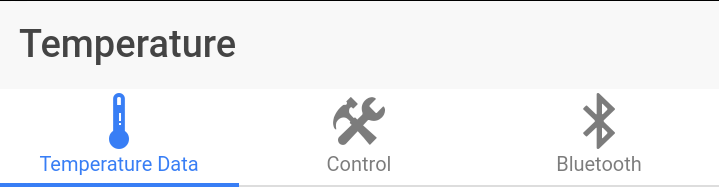
\includegraphics[scale=0.4]{pasekGora.png}
	\caption{Menu zakładek}
\end{figure}
Do przygotowania menu zakładek wykorzystano znaczniki \textit{<ion-tabs>}. Wyświetlenie treści odbywa się przez przełączanie widoku między stanami opisanymi na początku tego rozdziału.
\lstset{language=HTML}.
\begin{lstlisting}
<ion-tabs class="tabs-icon-top tabs-color-active-positive">
  <ion-tab title="Temperature Data" icon-off="ion-thermometer" icon-on="ion-thermometer" href="#/tab/temperature">
    <ion-nav-view name="tab-temperature"></ion-nav-view>
  </ion-tab>
  <ion-tab title="Control" icon-off="ion-settings" icon-on="ion-settings" href="#/tab/light">
    <ion-nav-view name="tab-light"></ion-nav-view>
  </ion-tab>
  <ion-tab title="Bluetooth" icon-off="ion-bluetooth" icon-on="ion-bluetooth" href="#/tab/bluetooth">
    <ion-nav-view name="tab-bluetooth"></ion-nav-view>
  </ion-tab>
</ion-tabs>
\end{lstlisting}
Do każdego z trzech przycisków przypisano nazwę i obrazek symbolizujący treść strony. Aktywna zakładka jest podświetlona w kolorze niebieskim.
\section{Strona pomiarowa}% jest ok
Strona pomiarowa służy wyłącznie do odczytu danych oraz ich wizualizacji. Struktura strony została zbudowana w sposób modułowy.
\begin{figure}[H]
	\centering
	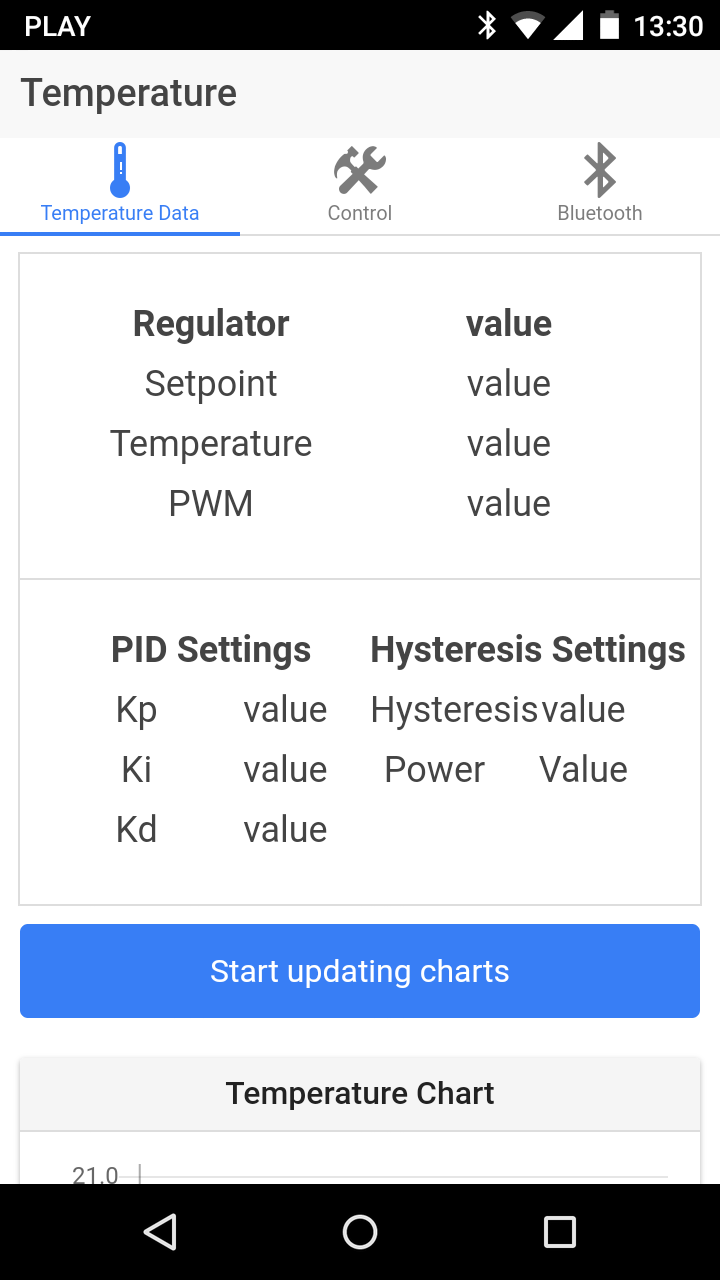
\includegraphics[scale=0.175]{apka1.png}
	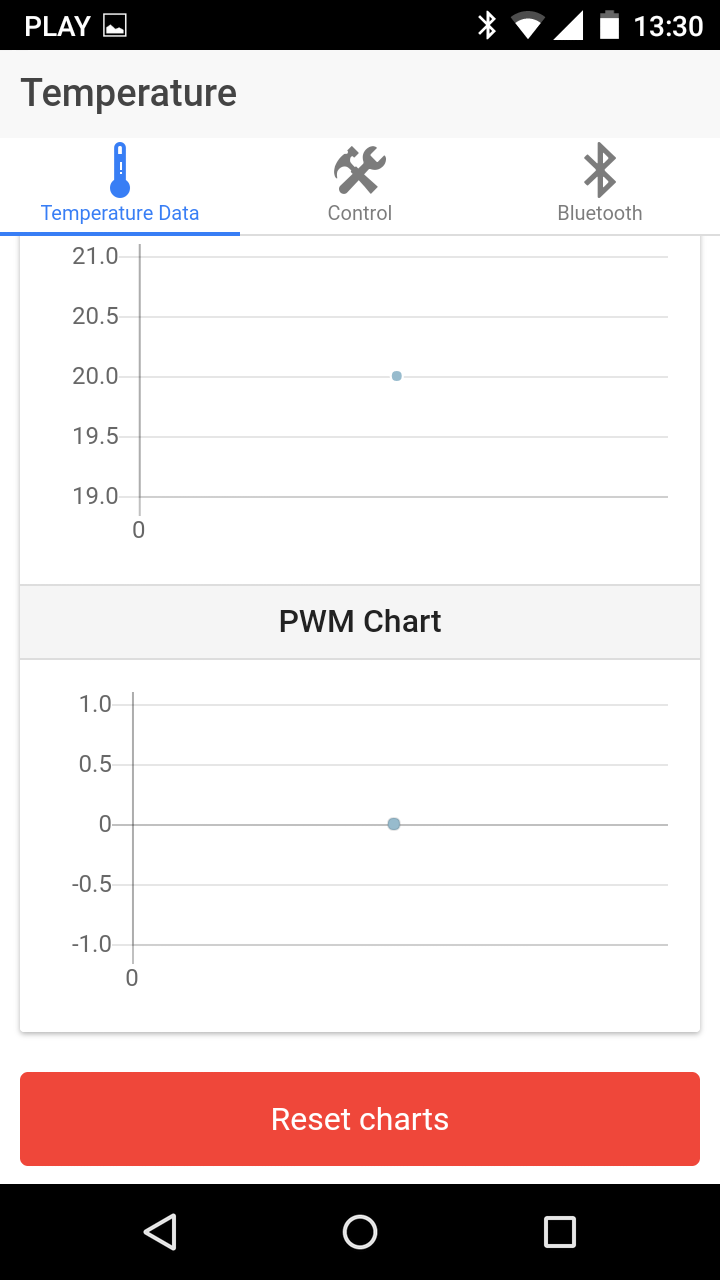
\includegraphics[scale=0.175]{apka2.png}
	\caption{Zakładka \textit{Temperature Data}}
\end{figure}
Podczas pracy układu regulacji bardzo ważna jest możliwość szybkiego odczytania aktualnych pomiarów i nastaw regulatorów. Dlatego, na początku zakładki umieszczono dwie tabele. Pierwsza z nich zawiera informacje ogólne, a druga specyficzne dla danego regulatora. Zamiast standardowych znaczników HTML, do utworzenia tabeli użyto znaczników \textit{div} oraz stylów mających odwzorować tabelę. Szerokość poszczególnych kolumn jest dopasowywana do wielkości wyświetlacza. Wyświetlane wartości zostały powiązane z kontrolerem \textit{TempCtrl} dzięki usłudze \textit{scope}. Takie rozwiązanie pozwala na uaktualnianie ich, po odebraniu nowych danych. 

Proces regulacji temperatury może zająć od kilku do kilkunastu minut. Dane wyświetlane w tabeli nie przekażą użytkownikowi informacji o tym, jak przebiegał proces w ostatnim okresie czasu. Za najciekawsze rozwiązanie uznano wizualizację danych na dwóch wykresach. Pierwszym przedstawiającym temperaturę aktualną i zadaną, a drugi sygnał sterujący PWM.
\begin{lstlisting} 
  <div class="card">
    <div class="item item-divider">
      Temperature Chart
    </div>
    <div class="item item-text-wrap">
      <canvas id="line1" class="chart chart-line" chart-data="data1" chart-labels="labels1" chart-legend="true" chart-series="series1" chart-options="options1"></canvas>
    </div>
    <div class="item item-divider">
      PWM Chart
    </div>
    <div class="item item-text-wrap">
      <canvas id="line2" class="chart chart-line" chart-data="data2" chart-labels="labels2" chart-legend="true" chart-series="series2" chart-options="options2"></canvas>
    </div>
  </div>
  <button class='button button-block button-assertive' ng-click="resetChart()">
    Reset charts
  </button>
\end{lstlisting}
Wykresy są dynamicznie aktualizowane, co trzecią pobraną próbkę danych. Ilość danych na wykresach ograniczono do 150 próbek, pozwalających na czytelne przedstawienie przebiegu procesu w ostatnich minutach. Po przekroczeniu zadanej ilości punktów, najstarsza informacja zostaje usunięta z wykresu. Do wyświetlenia grafów użyto znaczników \textit{<canvas>}, pozwalających na rysowanie wykresów przez JavaScript. Opcje dotyczące wykresów zostały sprecyzowane w kontrolerze strony.Ostatnim elementem strony jest przycisk \textit{Reset charts}, pozwalający na usunięcie wszystkich danych wyświetlonych na wykresach.

\subsection{Kontroler TempCtrl}%jest ok
TempCtrl to kontroler odpowiadający za możliwość ingerencji w interfejs użytkownika na stronie \textit{Temperature Data}. Odpowiedzialny jest za aktualizację wyświetlanych danych. W kontrolerze wykorzystano usługi:
\begin{itemize}
\item \textit{\$scope}- odpowiedzialny za połączenie kontrolera z widokiem użytkownika,
\item \textit{\$interval}- pozwala na wykorzystanie timerów,
\item \textit{receivedData}- serwis wykorzystywany do pobierania informacji,
\item \textit{bluetoothInformation}- serwis zawierający informację o aktualnym połączeniu Bluetooth.
\end{itemize}
Podobnie jak program mikrokontrolera Arduino, blok kontrolera posiada kod, który zostaje wykonany tylko raz, zaraz po pierwszym otwarciu zakładki. Wszystkim wyświetlanym parametrom, nadano wartość początkową \textit{value}. Sytuację przed pobraniem pierwszych próbek danych można zaobserwować na rysunku 6.1.
\lstset{language=Java}
\begin{lstlisting} 
	$scope.labels1 = [timeX];
	$scope.series1 = [['Actual Temperature'],['Setpoint']];
	$scope.data1=[[22],[22]];
	$scope.colors = ['#ff6384','#ff6384'];

	$scope.labels2 = [timeX];
	$scope.series2 = ['PWM'];
	$scope.data2=[0];
	$scope.color2 = ['#ff6384'];
\end{lstlisting}
W celu zainicjowania wykresów, wprowadzono na nie pierwszy punkt pomiarowy z aktualnym czasem i wartością mieszczącą się w zakresie pracy. Dodatkowo określono nazwy i kolory serii danych. Modyfikacja wyglądu wykresów nastąpiła poprzez przypisanie opcji do zmiennych \textit{\$scope.options} każdego wykresu. Oś Y umieszczono po lewej stronie. Ilość etykiet na osi X ograniczono do 4. W celu poprawienia płynności działania wykresów, wyłączono funkcję animacji rysowania nowego punktu.
\begin{lstlisting} 
	var interval1=$interval(receiveData, 1000);
\end{lstlisting}
Uruchomiony został również jedyny interwał wykonywany w tym kontrolerze. Funkcja \textit{receiveData} wykorzystuje usługę receivedData do pobrania nowych pomiarów z bufora modułu Bluetooth. Działanie cyklicznie wykonywanej funkcji zaczyna się od wykonania metody \textit{receivedData.getData()}, która pobiera i przetwarza dane. Następnie warunek \textit{if} sprawdza czy, odebrana paczka danych była kompletna. Jeśli tak, to wyświetlane wartości zostają zaktualizowane przy użyciu metod \textit{getKp, getTemperature} itd. Informacja o aktualnie pracującym regulatorze zostaje odebrana w postaci liczby, która w zależności od wartości zostaje zamieniona na tekst \textit{Hysteresis} lub \textit{PID}. Na końcu program sprawdza czy, było to już trzecie wywołanie funkcji aktualizacji. Jeśli tak, to zmienna licząca jest zerowana, a następnie proces przechodzi do wykonania funkcji \textit{updateCharts}. W przypadku otrzymania niepoprawnych danych, proces aktualizacji zostaje pominięty.

Na początku działania funkcji \textit{updateCharts()}, aktualizowana jest zmienna \textit{timeX} przechowująca aktualny czas. Przed dodaniem nowego punktu, sprawdzana jest ilość danych na wykresie. Jeśli jest ona równa lub większa 150, to należy usunąć najstarszą narysowaną próbkę z obu wykresów. Metoda \textit{slice} wycina tablicę z pominięciem jej pierwszej komórki i zapisuje ją zamiast starej zmiennej. Działanie zostaje powtórzone dla każdej serii danych obu wykresów. Następnie do tablicy dopisane zostają najświeższe pomiary używając metody \textit{push}.

Do przycisku \textit{Reset charts} za pomocą zdarzenia \textit{ng-click} przypisano funkcję \textit{resetChart} nadpisującą zestawy danych każdego z wykresów, ostatnio pobranymi wartościami.

\section{Zakładka konfiguracyjna}%jest ok
Zakładka konfiguracyjna została utworzona w celu możliwości wygodnego zmieniania temperatury zadanej, wyboru typu regulatora i jego nastaw. Wybrane ustawienia zostają przesłane do układu mikroprocesorowego, po użyciu przycisku \textit{Confirm new setting}.

Strukturę strony ponownie oparto o style dostępne w frameworku. Panel wyboru typu regulatora został utworzony za pomocą klasy \textit{item-select} i znaczników \textit{<select>}, do których przy pomocy polecenia \textit{ng-model} przypisano zmienną widoczną dla kontrolera tej karty.
\begin{figure}[H]
	\centering
	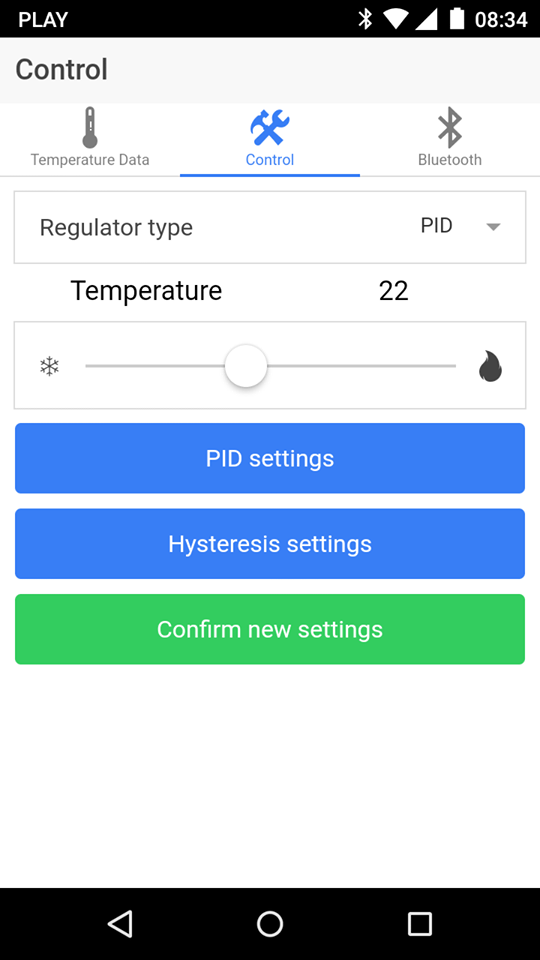
\includegraphics[scale=0.25]{apka3.png}
	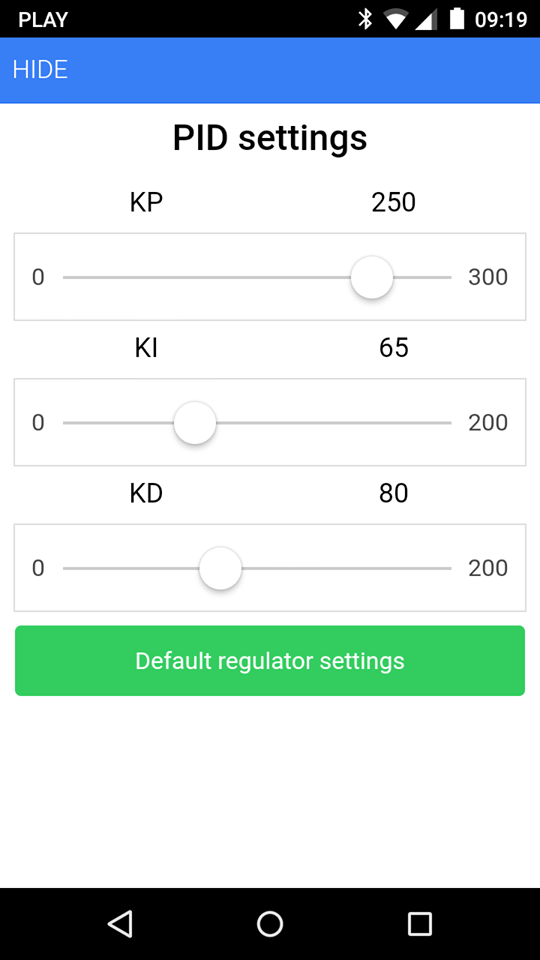
\includegraphics[scale=0.25]{apka4.png}
	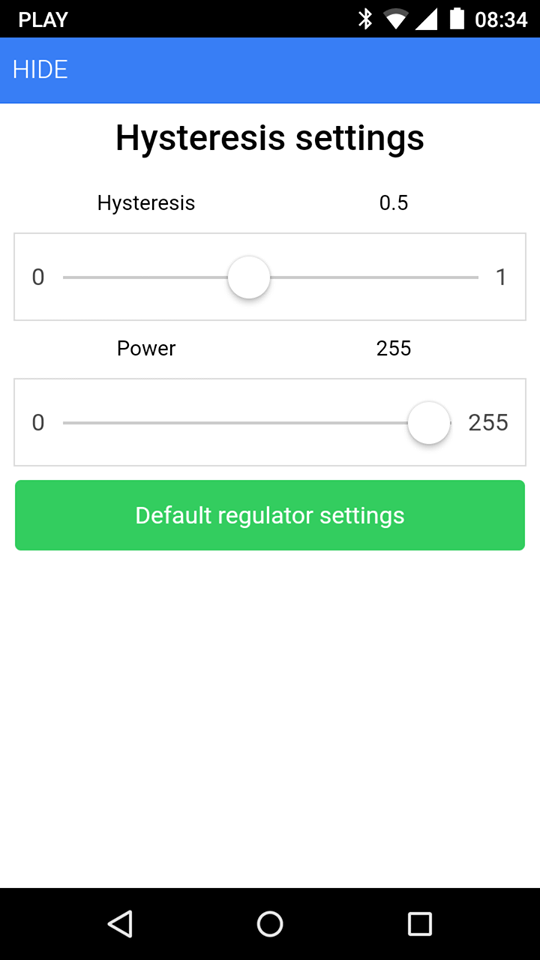
\includegraphics[scale=0.25]{apka5.png}
	\caption{Zakładka \textit{Control}}
\end{figure}


Za pomocą znacznika \textit{<input>} typu \textit{range} utworzono suwak regulacji temperatury zadanej. Po lewej stronie suwaka umieszczono ikonę płatka śniegu oznaczającego niską temperaturę, a z prawej strony płomień oznaczający wysoką temperaturę.

Kolejnymi elementami interfejsu są 2 przyciski. Każdy z nich otwiera nowy \textit{modal}. \textit{Modal}, to nowe okno widoku, pojawiające się nad głównym interfejsem użytkownika. Pierwszy z przycisków tworzy \textit{modal}, w którym ponownie umieszczono suwaki konfiguracji wzmocnień \textit{kp}, \textit{ki} i \textit{kd} regulatora PID. Pod suwakami umieszczono przycisk \textit{Default regulator settings}, pozwalający na przywrócenie standardowych nastaw regulatora. Modal odpowiadający drugiemu przyciskowi, został zaprojektowany w podobny sposób, ale zawiera on parametry regulatora histerezowego. Trzeci obiekt to przycisk potwierdzenia ustawień, który został wyróżniony zielonym kolorem. Zaakceptowanie ustawień jest potwierdzane komunikatem.

Struktura użytych \textit{modali} została zapisana w pliku HTML tej zakładki. Każdemu z nich został przydzielony indywidualny numer \textit{id}.

\subsection{Kontroler ControlCtrl} %jest ok
W celu poprawnego działania kontrolera użyto w nim usługi \textit{\$scope} oraz \textit{\$ionicModal}. Na początku bloku kontrolera utworzono zmienne powiązane z widokiem aplikacji, odpowiedzialne za wartości konfigurowane za pomocą suwaków i panelu wyboru. Ze względu na sposób działania wejścia w postaci suwaka, dane musiały zostać zapisane w  postaci obiektowej.
\begin{lstlisting} 
	var regulator=1;
	$scope.data={'regulatorType':'PID'};
	$scope.data1={'newSetpoint':'22'};
	$scope.data2={'kp':'15'};
	$scope.data3={'ki':'5'};
	$scope.data4={'kd':'2'};
	$scope.data5={'hyst':'0.25'}
	$scope.data6={'power':'255'}
\end{lstlisting}
Do zmiennych \textit{oModal1} i \textit{oModal2} przypisano modale utworzone w pliku HTML tej strony. Do zidentyfikowania ich został wykorzystany parametr \textit{id}.

Do przycisków odpowiedzialnych za wyświetlanie nowych okien, przypisano funkcję \textit{openModal()}, przyjmującą jako argument numer okna do otwarcia. Dla argumentu równego 1 zostaje otwarty widok konfiguracji regulatora PID, a dla 2 okno regulatora histerezowego. Wydarzeniem wykonywanym po naciśnięciu przycisku \textit{Hide} znajdującego się w lewym, górnym narożniku jest funkcja \textit{closeModal()}, przyjmująca te same argumentu co w poprzednim przypadku. Okno zostaje ukryte dzięki metodzie \textit{hide()}. Podczas otwierania użyto \textit{show()}.

Szczególną rolę w tym kontrolerze pełni funkcja \textit{sendSetpoint()}, odpowiedzialna za przesłanie ramki przedstawionej na rysunku 5.2. W celu ograniczenia ilości przesyłanych znaków, nazwa regulatora zostaje zastąpiona przez cyfrę.
\begin{lstlisting}
bluetoothSerial.write("t"+$scope.data1.newSetpoint+"p"+$scope.data2.kp+"i"+$scope.data3.ki+"d"+$scope.data4.kd+"r"+regulator+"h"+$scope.data5.hyst+"m"+$scope.data6.power+"/n")
\end{lstlisting}
Ramka zostaje wysłana za pomocą metody \textit{bluetoothSerial.write}, w przedstawiony powyżej sposób.. W przypadku pozytywnie zakończonego procesu wysyłania danych, zostaje wyświetlony komunikat, informujący o przesłaniu danych. W przeciwnej sytuacji wyświetlone okno informacyjne zawiera komunikat o niepowodzeniu przesyłania danych.

\section{Bluetooth}
Ostatnia utworzona zakładka służy do konfiguracji modułu Bluetooth urządzenia mobilnego. Kontroler utworzony do obsługi wydarzeń na stronie, nazywa się \textit{BlueCtrl}. Interfejs składa się na przycisk wyszukiwania urządzeń oraz dwie sekcje:
\begin{itemize}
\item urządzenia sparowane z telefonem,
\item nowe wyszukane urządzenia.
\end{itemize}
\begin{figure}[H]
	\centering
	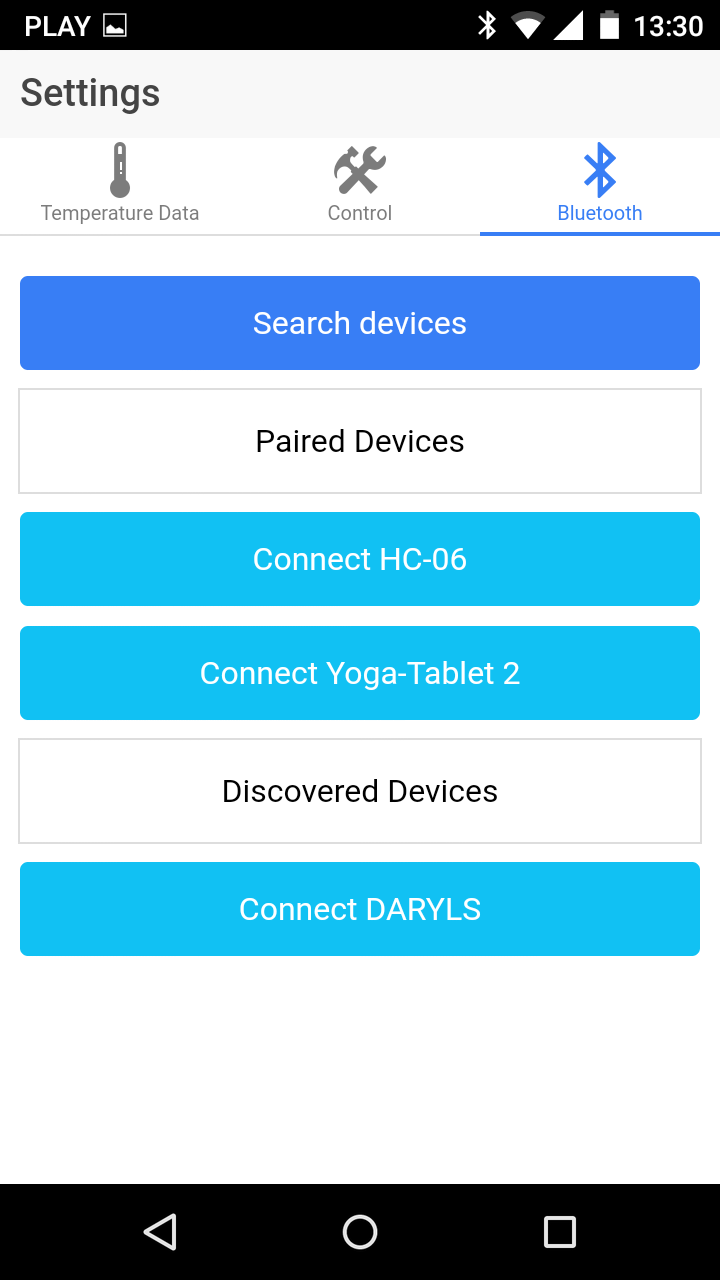
\includegraphics[scale=0.175]{apka6.png}
	\caption{Zakładka \textit{Bluetooth}}
\end{figure}
Program znajdzie wszystkie dostępne w okolicy urządzenia, ale nawiązanie komunikacji możliwe jest jedynie z modułem slave, podłączonym do Arduino. Do przycisku przypisano wydarzenie \textit{ng-click}, odwołujące się do funkcji \textit{findDevices()}, która została szerzej opisana w rozdziale poświęconym kontrolerowi \textit{BlueCtrl}. 
\lstset{language=HTML}
\begin{lstlisting}
<button ng-repeat="device in pairedDevices" ng-click="connectMac({{device}})" class='{{typeConnect}}'>
	{{textConnect}} {{device.name}}
</button>
\end{lstlisting}
W pliku HTML utworzono dwa przyciski, które początkowo są niewidoczne, dlatego że przypisane im obiekty nie zawierają jeszcze żadnych elementów. Po użyciu przycisku wyszukiwania, obiekty zostają wypełnione znalezionymi urządzeniami. Za pomocą dyrektywy \textit{ng-repeat} utworzony szkielet przycisku zostaje powielony dla każdego obiektu w obiekcie. Następnie każdy przycisk zostaje zidentyfikowany przez nazwę i adres urządzenia.

Po wciśnięciu wygenerowanego przycisku wywołana zostaje funkcja \textit{connectMac()}, przyjmująca jako argument obiekt, przypisany do przycisku.


\subsection{Kontroler BluetoothCtrl}


W celu dodatkowego zabezpieczenia poprawnej funkcjonalności aplikacji poza standardowymi usługami \textit{\$scope} i \textit{\$timeout}, użyto jeszcze serwisu \textit{\$ionicLoading} i \textit{bluetoothInformation}. Po uruchomieniu zakładki po raz pierwszy, powstają zmienne przechowujące bazowy wygląd przycisku połączenia z urządzeniem. Następnie po opóźnieniu równym 0.5 sekundy zostaje wykonana metoda \textit{bluetoothInformation.isBluetoothON()}, sprawdzająca czy moduł jest uruchomiony. Funkcja została opóźniona dlatego, że  wtyczka \textit{bluetoothSerial} jest dostępna dla aplikacji z minimalnym opóźnieniem. W przeciwnym wypadku metoda usługi zostały nierozpoznana.

Funkcja odpowiedzialna za wyszukiwanie nowych urządzeń została zabezpieczona przez warunek \textit{if}, ponownie sprawdzający czy moduł jest uruchomiony. Jeśli zostanie zwrócona wartość pozytywna, to ekran zostaje zablokowany przez proces wczytywania uruchomiony przez usługę \textit{\%ionicLoading}.  Zastosowano takie rozwiązanie w celu uniknięcia sytuacji, w której użytkownik wielokrotnie używa przycisku, zamiast zaczekać, aż funkcja zakończy pracę.

\begin{lstlisting}
bluetoothSerial.list(function (data) {
	console.log("List: "+data);
	$scope.$apply(function () {
		$scope.pairedDevices=data})},function () {
		console.log("No devices found");
	});
\end{lstlisting}
Lista wygenerowana przez metodę \textit{bluetoothSerial.list()} zostaje przekazana w formie argumentu \textit{data} do kolejnej funkcji. Otrzymane dane zapisane są w postaci obiektowej.Metoda wyszukująca dostępne urządzenia działa dokładnie w ten sam sposób. Po wykonaniu drugiej komendy, niezależnie od poprawności jej wykonania, ekran zostaje odblokowany. Dla zapewnienia poprawności działania aplikacji, a dokładniej wyświetlenia przycisków, aktualizacja uzyskanych danych do DOM, zostaje wymuszona przez polecenie \textit{\$scope.\$apply}.

Kolejną ważną funkcją powiązaną z elementami strony HTML jest polecenie \textit{connectMac(obiekt)}, które jako argument przyjmuje obiekt opisujący dane urządzenie. Po wywołaniu wydarzenia, ekran zostaje ponownie zablokowany. Następnie wykonywana jest usługa sprawdzająca status połączenia. W kolejnym kroku warunek \textit{if} sprawdza zwróconą wartość, opisującą status połączenia. Cześć usługi wykonującej funkcję sprawdzenia i część zwracająca wynik rozdzielono na dwie osobne metody ze względu na pojawiające się opóźnienie w przypisaniu danych. W zależności od spełnienia lub nie warunku, zostaje wywołana część bloku odpowiedzialna za rozłączenie z urządzeniem lub połączenie z nim. Każda uzyskana odpowiedź powoduje wyświetlenie się alertu informującego o wyniku przeprowadzonej operacji. W przypadku pozytywnego skutku rozłączenie lub niepowodzenia w połączeniu, zostaje wywołana funkcja \textit{checkConnection1()}, zmieniająca wygląd przycisków do postaci początkowej. Dla niepowodzenia w rozłączeniu i prawidłowego nawiązania połączenia zostaje wykonana funkcja \textit{checkConnection()}, która za pomocą usługi \textit{bluetoothInformation} sprawdza status połączenia i dopasowuje do niego wygląd przycisków. Następnie ekran aplikacji zostaje odblokowany.

